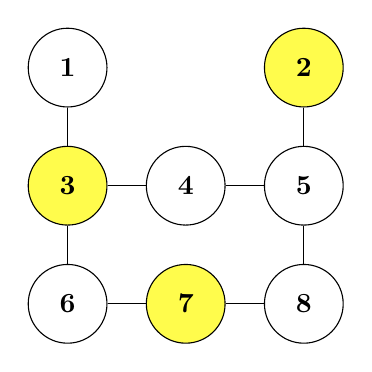
\begin{tikzpicture}[x=1.5cm, y=1.5cm]
  % 設定
  \tikzset{node/.style={circle,draw=black,minimum size=1cm}}
 
  % 色
  \definecolor{yellow}{RGB}{255,251,0}
 
  % 補助線
  % \draw [help lines,blue] (0,0) grid (20,6);
 
  % node %
  \node[node] at (-1,1) (node1) {\textbf{1}};
  \node[node, fill=yellow!70] at (1,1) (node2) {\textbf{2}};
  \node[node, fill=yellow!70] at (-1,0) (node3) {\textbf{3}};
  \node[node] at (0,0) (node4) {\textbf{4}};
  \node[node] at (1,0) (node5) {\textbf{5}};
  \node[node] at (-1,-1) (node6) {\textbf{6}};
  \node[node, fill=yellow!70] at (0,-1) (node7) {\textbf{7}};
  \node[node] at (1,-1) (node8) {\textbf{8}};
 
  \foreach \u / \v in {node1/node3, node2/node5, node3/node4, node3/node6, node4/node5,
    node5/node8, node6/node7, node7/node8}
  \draw (\u) -- (\v);
\end{tikzpicture}
